\documentclass[english,12pt,twoside]{article}

%% LyX 1.1 created some parts of this file.  For more info, see http://www.lyx.org/.
%% Do not edit unless you really know what you are doing.

\usepackage[T1]{fontenc}
\usepackage[nomarginpar]{geometry}
\usepackage{tocloft} %Allow us to leave page numbers for Parts out of table of contents
\cftpagenumbersoff{part} %No page numbers for Parts out of table of contents
\renewcommand{\cftsecdotsep}{\cftsubsecdotsep}
%\usepackage{newclude} %Allows use of /include*{}
%DANGER DANGER: newclude is NOT compatible with package xr, used for external references.
\geometry{verbose,letterpaper}
\usepackage{fancyhdr}
\usepackage{babel}
\setlength\parskip{\medskipamount}
\setlength\parindent{0pt}
\usepackage{graphicx}
\usepackage{wrapfig}
\usepackage{microtype} % (apparently not compatible with pdflatex)
%\usepackage{epstopdf} %this package apparently allows pdflatex to work on this document, since all we use are eps figures.
\usepackage{comment}
\usepackage{esvect}
\usepackage{amsmath} %uncommented by MT 5/2015, used in "E near charged rod"
\usepackage{amssymb}
\usepackage{mathtools} %added by MT 6/2015, for access to dcases environment in finding_v_from_e
\usepackage{tabularx} %added by MT 6/2015, for fixed width columns, used in rc_circuits
\usepackage{titlesec}
\usepackage{xr}
\usepackage{makeidx}
\usepackage{enumitem} %added 3/2016 by MT.  Tested 100% with other labs, looks like it does no harm.
%enumitem package allows enumerate[resume], which allows enumerate to play nicely with wrapfig (see induction1).
%enumitem package also provides very useful [wide] and [nosep] presets. (See, eg. resonance_tubes).
\usepackage{xcolor}
\usepackage[pagecolor={white},nopagecolor={white}]{pagecolor}

%For fixed width columns:
\newcolumntype{L}[1]{>{\raggedright\arraybackslash}p{#1}}
\newcolumntype{C}[1]{>{\centering\arraybackslash}p{#1}}
\newcolumntype{R}[1]{>{\raggedleft\arraybackslash}p{#1}}


\addtolength{\oddsidemargin}{1.0cm} %without these two lines, larger margin is on the OUTSIDE.  We want the larger edge on the INSIDE, to allow room for the three hole punches
\addtolength{\evensidemargin}{-1.0cm}

\setlength\headheight{15pt}
\setlength\topmargin{0.2in}
\addtolength{\hoffset}{-1.0cm}
\addtolength{\textwidth}{2.0cm}
\addtolength{\voffset}{-1.5cm} %This line is apparently needed on some versions of MikTex XeLatex.  Comment out if your pages appear shifted too high.
\addtolength{\textheight}{3.5cm}
% define a strut for extra vertical space in tables.
\newcommand{\hi}{\rule[-2mm]{0mm}{6mm}}

\pagestyle{fancy}
%\fancyhead[LE,RO]{\slshape \rightmark} %This is the default for fancy page style
%\fancyhead[LO,RE]{\slshape \leftmark}
\fancyhead[LO,RE]{\slshape \rightmark} 
\fancyhead[LE,RO]{\slshape \leftmark} % Reversed LE, RO to  LO,RE to make headers come out correctly on even/odd pages



%%%%%%%%%%%%%%%%%%%%%%%%%%%%%% LyX specific LaTeX commands.
\providecommand{\LyX}{L\kern-.1667em\lower.25em\hbox{Y}\kern-.125emX\@}
\newenvironment{LyXParagraphIndent}[1]%
{
  \begin{list}{}{%
    \setlength\topsep{0pt}%
    \addtolength{\leftmargin}{#1}
    \setlength\parsep{0pt plus 1pt}%
  }
  \item[]
}
{\end{list}}
%% Special footnote code from the package 'stblftnt.sty'
%% Author: Robin Fairbairns -- Last revised Dec 13 1996
\makeatletter
\let\SF@@footnote\footnote
\def\footnote{\ifx\protect\@typeset@protect
    \expandafter\SF@@footnote
  \else
    \expandafter\SF@gobble@opt
  \fi
}
\expandafter\def\csname SF@gobble@opt \endcsname{\@ifnextchar[%]
  \SF@gobble@twobracket
  \@gobble
}
\edef\SF@gobble@opt{\noexpand\protect
  \expandafter\noexpand\csname SF@gobble@opt \endcsname}
\def\SF@gobble@twobracket[#1]#2{}
\makeatother


%I make use of some latex features to manage the section numbers. To use those you have to insert the following lines into the latex preamble (before the %"\begin{document}" command).

% two new commands to do labelling. - gpg 12/4/13
\newcommand{\customlabel}[2]{%
\protected@write \@auxout {}{\string \newlabel {#1}{{#2}{}}}}

\newcommand{\actlabel}[1]{%
\protected@write \@auxout {}{\string \newlabel {#1}{{\arabic{activity}}{}}}}

\newcommand{\makelabheader}
%{Name: \rule{2.0in}{0.1pt}\hfill{}Section: \rule{1.0in}{0.1pt}\hfill{}Date: \rule{1.0in}{0.1pt}}
{Name: \rule{2.0in}{0.1pt}\hfill{}Lab Partner(s): \rule{3.0in}{0.1pt}}

%\newcommand{\dir131}{../../131/StudentGuideModule1} %This does not work, because commands can only be made of numeric characters, not numbers.

%A new command for putting a box around a paragraph:
\newenvironment{newboxed} %maybe there's a better way to do this.  I just cribbed from the web. --MT
    {\begin{center}
    \begin{tabular}{|p{0.9\textwidth}|}
    \hline\\
    }
    { 
    \\\\\hline
    \end{tabular} 
    \end{center}
    }

\newcounter{activity}

%  The following command, \answerspace, should be used to replace \vspace.
%  \vspace{} is not ideal for an answer space for students, for two reasons:
%  1. It can be ignored if it comes at the end of a page, and
%  2. The spacing is exact, and Latex will not stretch or compress it at all to make things fit on a page, which means
%  that other things WILL get stretched or compressed to make things fit, which means those other things will 
%  end up looking bad, and leading to a lot of underfull \vbox warnings.
%  \answerspace fixes both of those problems, specifically allowing the space to grow to up to 1.5 times the stated size.

\newlength\answerlength
\newcommand{\answerspace}[1]{
	\setlength\answerlength{#1}
	\vspace*{1.0\answerlength plus 0.5\answerlength}}

%  The next several lines implement \includelab, which replaces \include.
%  Usage is \includelab{1}{file} to include it, or \includelab{0}{file} to NOT include it.  
%  But all 0's can be overridden by writing \includealllabstrue in the master.tex file, which is easier than deleting 
%  fifty individual `%' signs and then remembering to put them all back, which is what you had to do before.
%  \includeonly still works as you expect it to.
\newif\ifincludealllabs
\newcommand{\includelab}[2]{
	\ifnum#1=1
		\include{#2}
	\else {
		\ifincludealllabs
		 	\include{#2}
		\fi}
	\fi
}
 %all general latex packages, commands, and definitions now here.

%The \includeonly line below is a great way to save time so you don't always have to compile the WHOLE latex document, if for instance you've only made changes to a single lab.  If you want to compile more than two labs, the syntax is \includeonly{lab1,lab2,lab3} with no spaces after the commas.
%The master.pdf produced will have only the title page, TOC, and that single lab, though the other lab names will appear in the TOC.
%\includeonly{appendices/equipment/equipment}

%Use the following line to override all of the 1's and 0's in the \includelab statements below
%\includealllabstrue

\makeindex

\ForceSectionOddPage

\begin{document}

%\newgeometry{total={8in,10.5in},hoffset=0.2in,voffset=0.3in}
\newgeometry{total={8.5in,11in},hoffset=0in,voffset=0in}
%nb: I just messed with the numbers above until it looked okay.  I really don't know what I'm doing. --MT, 4/23/2016
\thispagestyle{empty}
\definecolor{darkblue}{RGB}{0,0,160}
\definecolor{lighterblue}{RGB}{0,128,255} %Looks better on the print shop's printer
\newpagecolor{lighterblue}

%\begin{center}\includegraphics[width=8.5in,trim={0 0 .1cm 0},clip]{electronics_front_pages/electronics_front_cover.eps}
\begin{center}\includegraphics[width=8.49in]{electronics_front_pages/electronics_front_cover_kuri.eps}

\index{color page}
\end{center}
\newpage

\restoregeometry
\restorepagecolor
\thispagestyle{empty}

\
\vfill
%\textit{Cover art: A randomly chosen, impressive-looking circuit.  You won't build one of these, but you'll do plenty of other cool stuff.}
\textit{Cover art: The circuit diagram from the final class project of a student who took this course in a previous year.  By the end of this course, you will understand all of the components in this diagram and will be able to design and build similar circuits  yourself.}
\pagebreak



\title{Electronics For Doing!\\
Laboratory Exercises for Physics 216}

\author{Matthew L. Trawick\\[4pt]
Department of Physics, University of Richmond, VA \\[4pt]
}

\maketitle

\vspace{0.4 in}

%\begin{abstract}

\begin{center}
\large{\textbf{Welcome to Electronics!}}
\end{center}

The exercises in this manual are for a course in electronics that emphasizes active learning. 
Sitting passively and listening to lectures is boring, and doesn't help you learn very well either.
Instead, this manual will guide you through a series of exercises designed to help you learn things by yourself as you go along, interrupted by me only occasionally to explain some of the tricky parts.

As you work, think about what you're supposed to be learning with each exercise.  If an exercise shows you a circuit that does X, then you should walk away from the lab knowing exactly how to build a circuit that does X.  Presumably, you'll be asked to do so on an exam soon enough!

Your written work will be done in a separate lab notebook.  For each numbered part, you should document your work with a quick circuit diagram or note about what you did, and include any data you take and any conclusions you draw.  Also, any sentence in this manual that ends with a question mark needs to be answered by you in your notebook.

Electronics is fun!  Don't be afraid to experiment!  The worst that can happen is you light some components on fire.  (No worries---they're not yours!)

Enjoy the ride and be excellent,

---Matt Trawick
%\end{abstract}


\newpage
\
\thispagestyle{plain}

\newpage
\




\tableofcontents{}
\cleardoublepage
\renewcommand{\headersupplementmark}{Lab }

%--------------------------------------------
\part{The Basics}

\includelab{1}{equipment/equipment}
\includelab{1}{power/power}
\includelab{1}{voltage_dividers/voltage_dividers}
\includelab{1}{input_output_impedance/input_output_impedance}
\includelab{1}{oscilloscope/oscilloscope}
\includelab{1}{bridge_circuit/bridge_circuit}

%--------------------------------------------
\part{Two Very Important Kinds of Integrated Circuits}

\includelab{1}{op-amps/op-amps}
\includelab{1}{digital_electronics/digital_electronics} %ADD pinouts sometime later

%--------------------------------------------
\part{Capacitors, Inductors, and AC circuits}

\includelab{1}{capacitors/capacitors}
\includelab{1}{transformers/transformers}
\includelab{1}{diodes/diodes}
\includelab{1}{power_supply/power_supply}
\includelab{1}{inductors/inductors}
\includelab{1}{ac_circuits/ac_circuits}
\includelab{1}{filters/filters}

%--------------------------------------------
\part{Relays and Transistors}

\includelab{1}{relays/relays}
\includelab{1}{bjt/bjt}
\includelab{1}{multisim/multisim}
\includelab{1}{bjt_saturation/bjt_saturation}
\includelab{1}{jfet/jfet}

%--------------------------------------------
\part{Sensors, Some Special Purpose Chips, and Applications}

\includelab{1}{microphone_photocell/microphone_photocell}
\includelab{1}{flipflops/flipflops}
\includelab{1}{timers/timers}
\includelab{1}{counters/counters}
\setcounter{section}{98} %set this to desired next section number MINUS ONE
\includelab{1}{lab_99/lab_99}

%--------------------------------------------
%\part{Appendices}
\immediateaddcontentsline{toc}{part}{Appendices} %Avoids a Roman part number for the Appendices in the toc
\appendix
\renewcommand{\headersupplementmark}{Appendix }
\titleformat{\section}{\normalfont\large\bfseries}{\headersupplementmark \thesection :}{1ex}{}

%\cleardoublepage
%\NoForceSectionOddPage

\includelab{1}{appendices/pinouts/pinouts}
\includelab{1}{appendices/one_page_uncertainty/one_page_uncertainty}
\includelab{1}{appendices/oscilloscope_checklist/oscilloscope_checklist}

\end{document}
